% -*- coding: utf-8 -*-

\section{Introduction}
\label{introduction}

The area of protein folding (and from this the creation of newer and better drugs) with the aid of computers, has since the 60's been an area of much research and experimentation. \Sfixme{Improve this part}

Since proteins cannot physically overlap with parts of itself, it is necessary that each conformation is tested for overlap before it the model commits to it. It is therefore critical that the overlap tests can be done quickly.

One method for detecting collisions is Bounding Volumes Hierarchy (BVH), using a Bounding Volume (BV), where each node in the BVH is enveloped by a BV that covers all the children of the nodes\footnote{The leafs of the node is a small group of atoms}. If a BV does not intersect any other BV, then it is clear that the attempted conformation is legal, and it can take place. If there is a overlap between, at least, two BVs, then further checks (lower in the BVH) are needed, in order to validate whether there truly is an overlap.

\begin{figure}
\centering
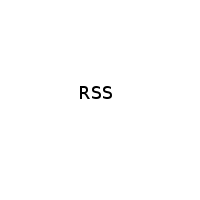
\includegraphics[width=0.5\textwidth]{figures/rss}
\caption{\label{rss-example-figure}An example of a RSS}
\end{figure}

One possible BV is the Rectangular Swept Sphere (RSS), which is generated by sweeping a sphere (with a positive radius) over a rectangle in 3D space. The resulting volume looks something like a pillow. An illustration is given in figure \ref{rss-example-figure}. 

\subsection{Scope and Limitations}
\label{scope}
I will in this project attempt to implement a RSS BV in the ProGAL framework. The RSS BV will contain the following 3 methods:

\begin{description}
\item[Overlap detection:] In order to make it a viable BV for use in a BVH for protein folding, I will implement the overlap detection, which I have argued for and described in the last section. 

\item[Creation of RSS from a set of points:] In order to make the RSS viable for both testing and the BVH, I will implement a method that can construct a RSS from a set of points.
\item[Encapsulating RSS:] Lastly I will implement a method that will create a new RSS from any two given RSS'. This method is needed in for fast updates of the BVH, when a conformation happens in the protein.
\end{description}

Of these 3 methods it is primarily the overlap and Encapsulating method where speed is of the essence.

I will not try to implement the RSS in the BVH. The reason for this is that it would take too long to implement it probably, compared to the utility it would bring to use the time on implementing the RSS and the other methods properly. It will however mean that I will not be able to test my implementation by  actively folding of proteins, though I will test it on provided test data derived from snapshots of proteins.

\subsection{Expectations to the reader}
I expect the reader to have a good grasp of computational geometry, vector manipulations, and algorithms in general.

\subsection{Terminology}
In this report I will use the term ``good fit'' to mean that the Bounding Volume around a point-set contains all the points within it, and that it has as little wasted space - i.e. regions of the BV with no points in it as possible. BV A is a better fit than BV B, if both BV's a given set of points but A has a smaller volume than B.

\subsection{Guide to this report}
\begin{description}
\item[Section \ref{introduction}] The introduction to the report, which will introduce the subject and explain my goals
\item[Section \ref{rss}] A description of the Rectangular Swept Spheres - how they are defined in theory, and how I have chosen to represent them. This section will also contain information about the literature I have used in this report.
\item[Section \ref{algorithms}] The algorithms that work on the RSSs, and an analysis of their run time.
\item[Section \ref{implementation}] Notes on the implementation of the algorithms from the previous section and the RSS itself in ProGAL.
\item[Section \ref{results}] I will discus about the results and a comparison with Oriented Bounding Boxes. 
\item[Section \ref{conclusion}] The conclusion of the report, where I will sum up my findings, give some final critique of the literature I have used, as well as pointing to possible future work. 
\end{description}
